\documentclass{article}
\usepackage[utf8]{inputenc}
\usepackage{epigraph}
\usepackage{amsfonts}
\usepackage{amsmath}
\usepackage{graphicx}

\title{I teoremi del calcolo differenziale}
\author{V BC}
\date{}

\begin{document}

\maketitle
%\tableofcontents

\epigraph{``Il calcolo infinitesimale può essere considerato come un'applicazione della dialettica alle relazioni matematiche.” {--- \textup{F. Engels}}}

\section{Teorema di Fermat}

\subsection{Enunciato}

Sia $f(x)$ una funzione definita su un intervallo $(a,b)$, e sia $c \in (a,b)$ un punto estremante di $f$. Se $f$ è derivabile in $c$, allora $f'(c) = 0$.

\subsection{Note}

Il teorema di Fermat ci dice che (formulazioni equivalenti):
\begin{itemize}
    \item Se $c$ è estremante per $f(x)$, allora $f'(c) = 0$. Non è necessariamente vero l'opposto: infatti, si ha $f'(c) = 0$ anche se $c$ è un punto di flesso;
    \item Data una funzione $f(x)$ definita in un intervallo contenente il punto $c$, condizione necessaria ma non sufficente affinchè $c$ sia punto estremante è che sia punto stazionario, ossia che $f'(c)=0$.
\end{itemize}

\subsection{Dimostrazione}

Vedi quanto fatto in classe o libro p. 263. Sul libro, leggere ``ipotesi e tesi" p. 264 e ``non viceversa" p. 265. 

\section{Teorema di Rolle}

\subsection{Enunciato}

Sia $f(x)$ una funzione continua in un intervallo chiuso e limitato $[a,b]$, e derivabile al suo interno, ossia in $(a,b)$. Se $f(a) = f(b)$, allora esiste almeno un punto $c\in(a,b)$ tale che ivi la derivata si annulla: 

\begin{equation}
    f'(c) = 0
\end{equation}

\subsection{Dimostrazione}

Segui quanto riportato a p. 265-266. Passaggi essenziali:
\begin{enumerate}
    \item $f$ continua in intervallo chiuso e limitato $\rightarrow$ Weierstrass $\rightarrow$ la funzione ammette max ($M$) e min ($m$) assoluto
    \item $c,d$ punti di $[a,b]$ tali che $f(c) = M$, $f(d) = m$. Casi possibili:
    \begin{enumerate}
        \item $c=a$, $d=b$. I due punti $c$ e $d$ corrispondono con gli estremi di $[a,b]$. $f$ costante, $f'(c) = 0$ $\forall c \in [a,b]$;
        \item Almeno uno dei due punti (supponiamo si tratti di $c$) è interno ad $[a,b]$. Punto estremante interno al dominio $\rightarrow$ Teorema di Fermat $\rightarrow$ $f'(c) = 0$.  
    \end{enumerate}
\end{enumerate}

\subsection{Note}

Per il teorema di Rolle, nell'intervallo considerato la funzione ha {\emph{almeno}} un punto $c$ in cui si annulla. Ciò non esclude che ci possano essere {\emph{molteplici}} punti $\gamma$ tali che $f'(\gamma) = 0$.

Leggere e capire ``ipotesi e tesi" p. 267.

\begin{figure}
    \centering
    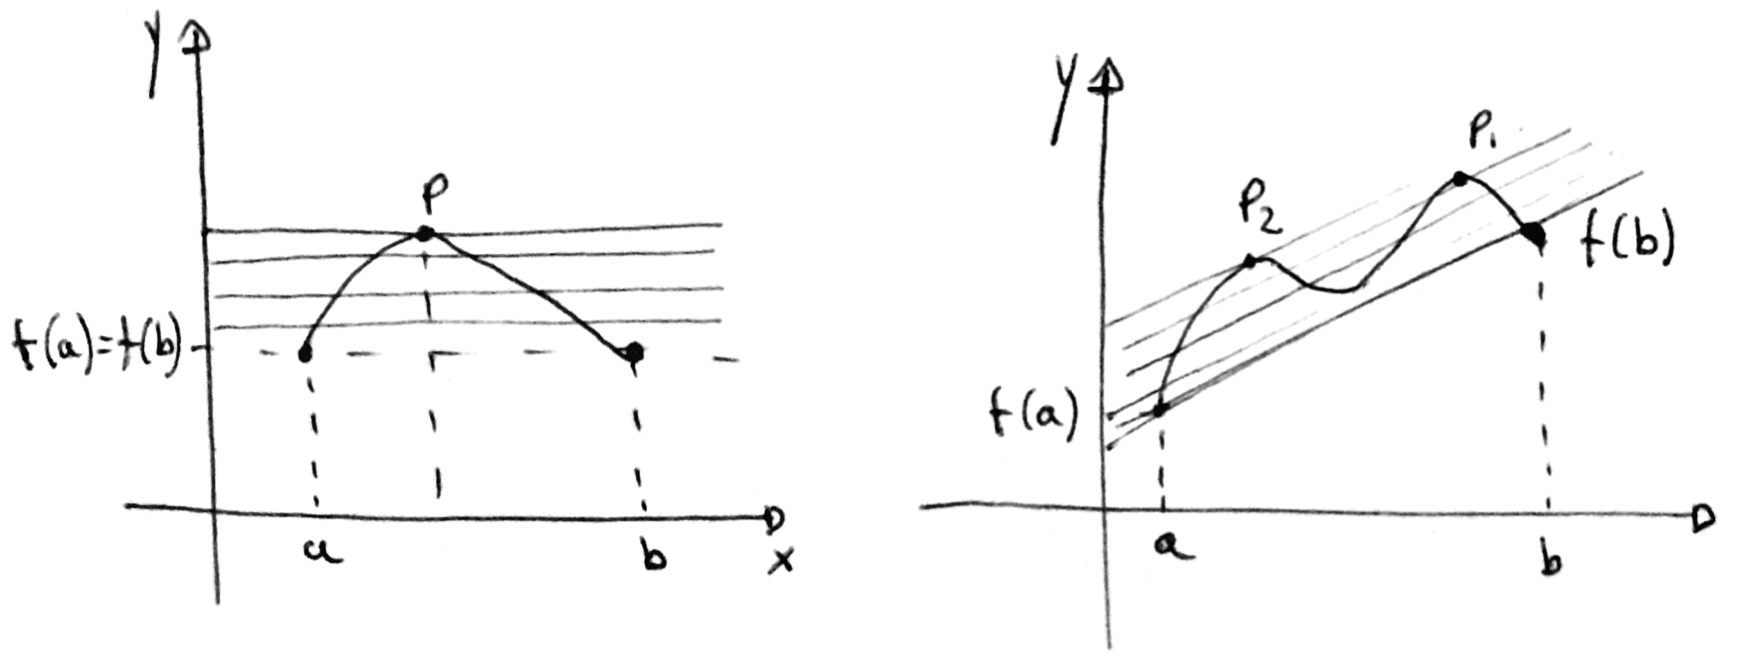
\includegraphics[width=0.9\textwidth]{Rolle_Lagrange.jpg}
    \caption{Rappresentazione grafica del significato del teorema di Rolle (sinistra) e del teorema di Lagrange (destra).}
    \label{fig:my_label}
\end{figure}

\section{Teorema di Lagrange\footnote{Nato Giuseppe Lodovico Lagrangia nel 1736 a Torino.}}

\subsection{Enunciato}

Sia $f(x)$ una funzione continua nell'intervallo chiuso e limitato $[a,b]$, e derivabile al suo interno. Allora esiste almeno un punto $c\in(a,b)$ tale che 

\begin{equation}
    f'(c) = \frac{f(b) - f(a)}{b-a}
\end{equation}

\subsection{Dimostrazione}

Data una costante $K\in\mathbb{R}$, possiamo definire la funzione

\begin{equation}
    \phi(x) = f(x) - Kx
    \label{dim_lagrange}
\end{equation}

Dato che $f(x) = x$ è una funzione continua e derivabile in $\mathbb{R}$, $\phi$ ha le stesse proprietà di $f$: è continua in $[a,b]$ e derivabile in $(a,b)$. Fissiamo $K$ in modo da poter applicare il {\emph{teorema di Rolle}}:

\begin{equation}
    \phi(a) = \phi(b) \rightarrow f(a) - Ka = f(b) - Kb \rightarrow K = \frac{f(b)-f(a)}{b-a}
\end{equation}

Per tale valore di $K$, Eq. \eqref{dim_lagrange} si può riscrivere come

\begin{equation}
    \phi(x) = f(x) -\frac{f(b)-f(a)}{b-a}x
\end{equation}

Da cui

\begin{equation}
    \phi'(x) = f'(x) -\frac{f(b)-f(a)}{b-a}
    \label{lagrange_derivata}
\end{equation}

Per il {\emph{teorema di Rolle}}, esiste $c\in(a,b)$ tale che $\phi'(c) = 0$. Di conseguenza, da Eq. \eqref{lagrange_derivata} si ha 

\begin{align}
    & 0 = f'(c) -\frac{f(b)-f(a)}{b-a} \\
    & f'(c) = \frac{f(b)-f(a)}{b-a}
\end{align}

\subsection{Note}

Possiamo considerare il teorema di Rolle come un caso particolare del teorema di Lagrange: infatti se $f(a) = f(b)$ (ipotesi del teorema di Rolle), 

\begin{equation}
    f'(x) = \frac{f(b)-f(a)}{b-a}
\end{equation}

Diventa 

\begin{equation}
    f'(x) = 0
\end{equation}

Come descritto dal teorema di Rolle. 

\section{Teorema di de l'H\^opital}

\subsection{Enunciato}

Siano $f(x)$ e $g(x)$ due funzioni continue in un intorno $U$ di $c$. Siano inoltre soddisfatte le seguenti ipotesi:
\begin{itemize}
    \item $f(x)$ e $g(x)$ sono derivabili in $U$ (tranne eventualmente $c$)
    \item $g'(x) \neq 0$ per tutti i punti di $U$ (tranne eventualmente $c$)
    \item Per $x\rightarrow c$, le due funzioni hanno entrambe limite zero o $\infty$
    \item Esiste, finito o infinito, $\lim_{x\rightarrow c} \frac{f'(x)}{g'(x)}$
\end{itemize}

Allora esiste anche $\lim_{x\rightarrow c} \frac{f(x)}{g(x)}$, e si ha:

\begin{equation}
    \lim_{x\rightarrow c} \frac{f(x)}{g(x)} = \lim_{x\rightarrow c} \frac{f'(x)}{g'(x)}
\end{equation}

\subsection{Note}

Grazie alla regola di de l'H\^opital, è possibile calcolare i limiti di rapporti di due funzioni che valgono $\frac{0}{0}$ o $\frac{\infty}{\infty}$.

\begin{figure}
    \centering
    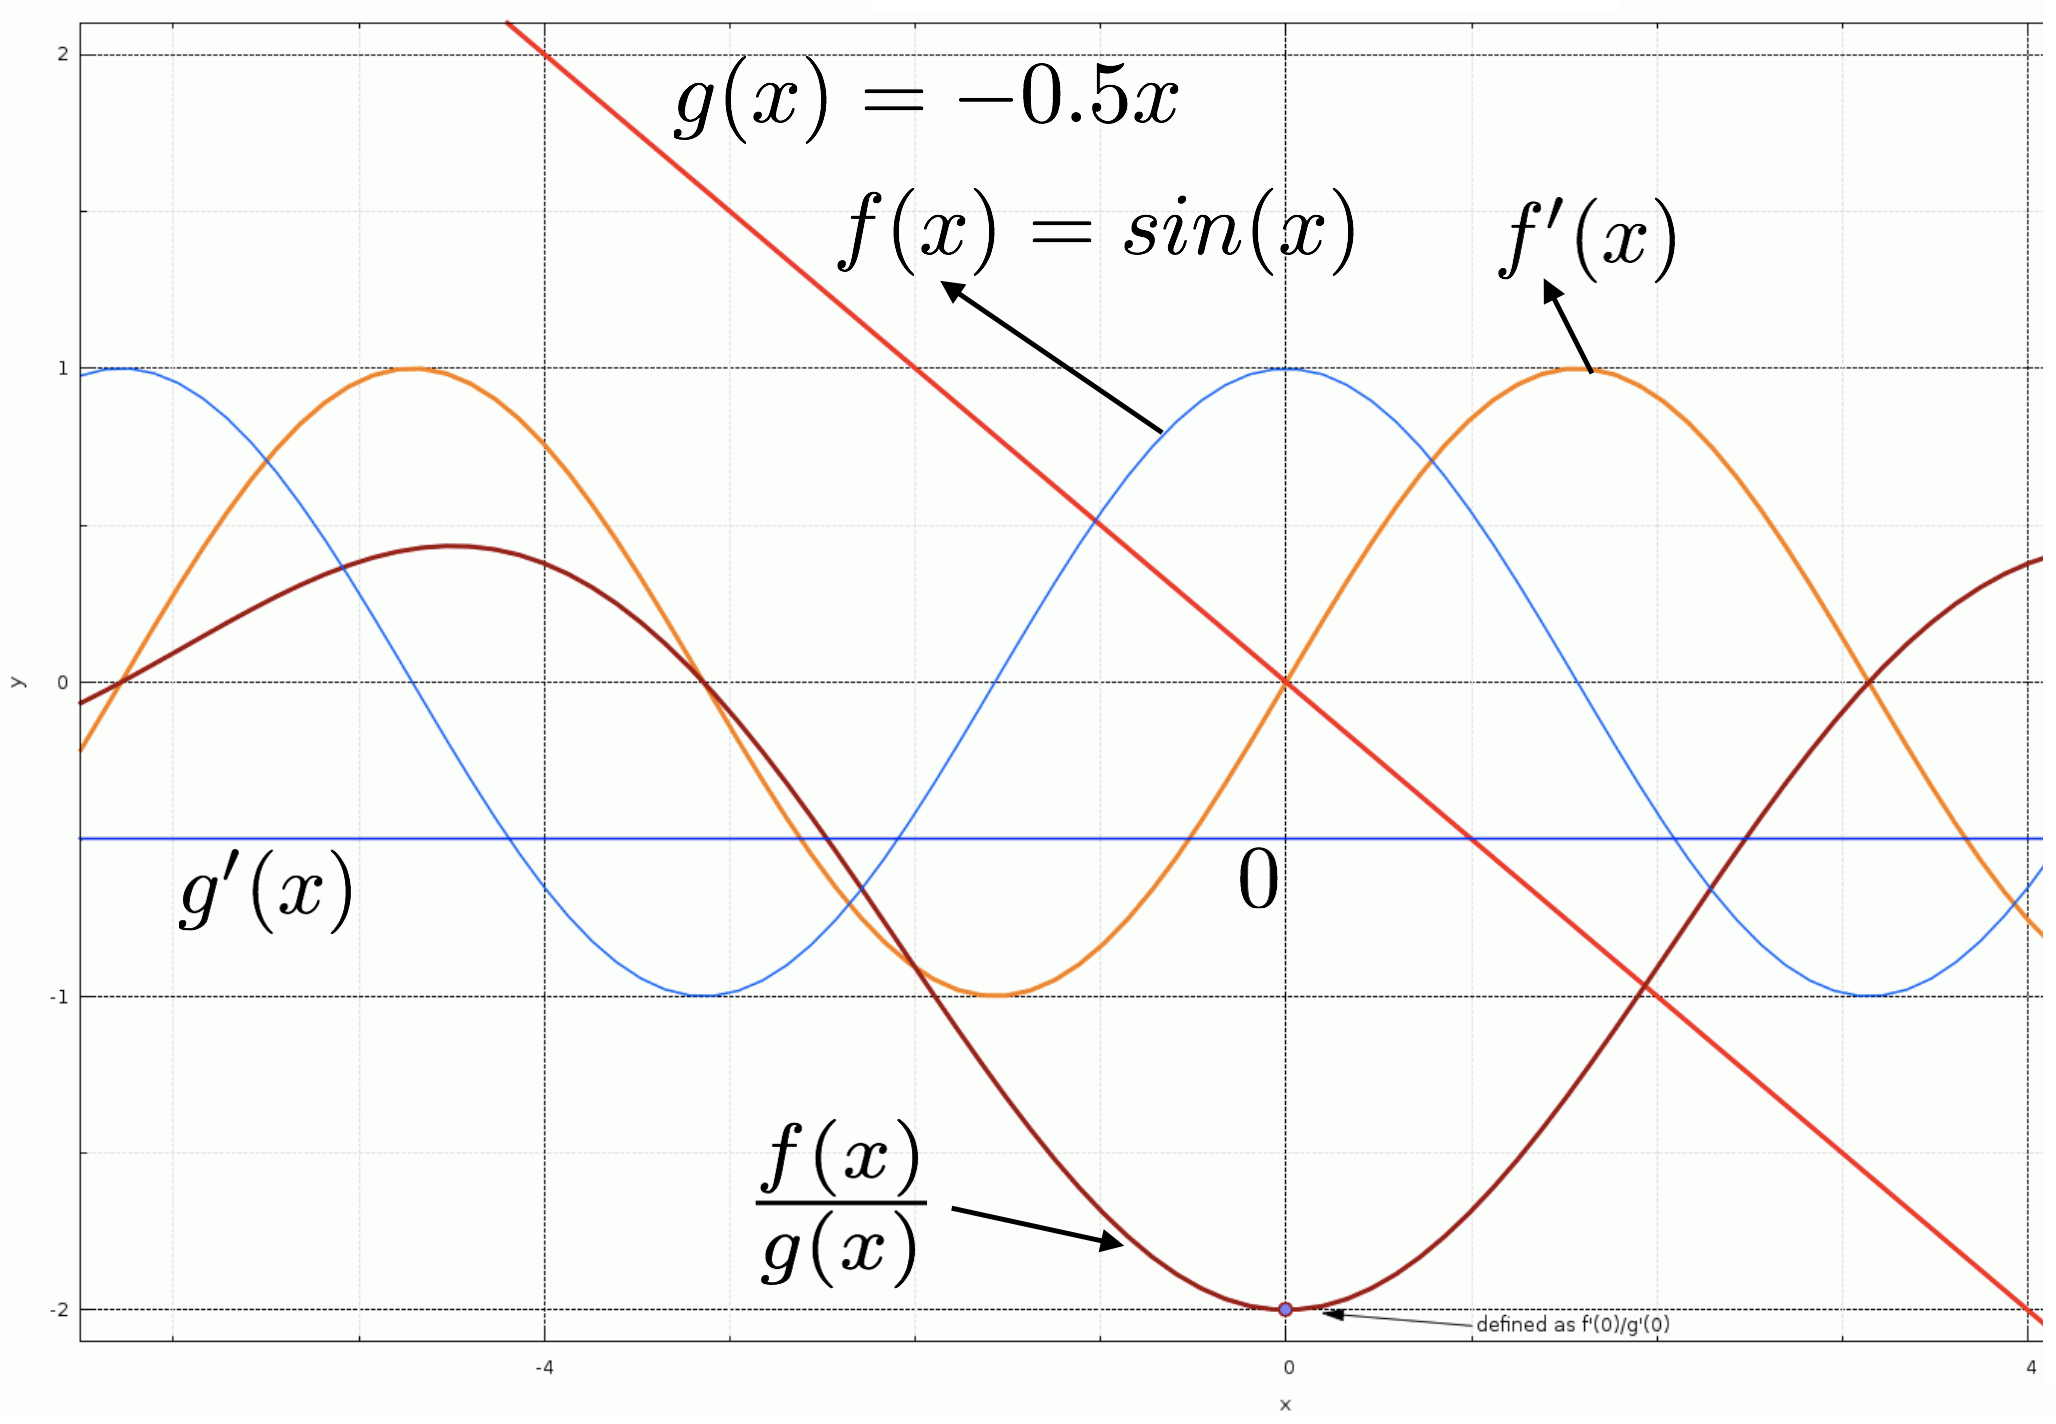
\includegraphics[width=0.8\textwidth]{Hospital.jpg}
    \caption{Esempio di applicazione del teorema di de l'H\^opital: la funzione $h(x) = \frac{f(x)}{g(x)} = -\frac{sin(x)}{0.5x}$ non è definita in $x=0$, ma il grafico può essere completato considerando $h'(x) = \frac{f'(x)}{g'(x)} = -\frac{cos(x)}{0.5}$, che è definita in 0.}
    \label{fig:my_label}
\end{figure}

\end{document}
